\chapter{Análisis del problema}
 
 Como todo software, esta aplicación se ha diseñado y desarrollado para cubrir una
 necesidad. En base a dicha premisa, podemos crear una descripción completa de los 
 actores así como una lista de requisitos detallada con la que se cubran los objetivos 
 propuestos.

\section{Descripción de los actores}
Vamos a disponer de dos actores: el \textbf{usuario} y el \textbf{administrador}.\\

El \textbf{usuario} será el agente de policía que desée realizar cualquiera de las acciones
disponibles en la aplicación. Este actor no tiene por qué tener ninguna experiencia previa
con aplicaciones web pero en este escenario se les ha formado con unas nociones básicas 
a modo de tutorial de como realizar todas las acciones posibles en la aplicación y las consecuencias
que tiene en el servidor.\\

El \textbf{administrador} será la persona encargada de asegurar el correcto funcionamiento 
del software así como el encargado de la gestión de los datos de usuario y de la aplicación. Este
actor, por tanto, debe tener un alto conocimiento de las tecnologías con las que se ha construido
\textbf{Chief} para poder dar una rápida respuesta a los posibles problemas del usuario.

\section{Análisis de requisitos}

Los requisitos serán divididos en 3 tipos:

\begin{itemize}
   \item \textbf{Requisitos funcionales:} Son servicios que el sistema debe proporcionar, cómo
   debería responder a entradas concretas y como debe reaccionar el sistema en situaciones 
   particulares. En algunos casos, se puede especificar explícitamente qué no debe hacer el sistema.

   \item \textbf{Requisitos no funcionales:} Son requisitos que no tienen que estar directamente relacionado
   con el funcionamiento de la aplicación sino más bien, con el proceso del desarrollo.
   
   \item \textbf{Requisitos de información:} Estos requisitos están relacionados con la información 
   que se va a guardar en el sistema.

   % Definiciones por: 
   % Chapter 6. Ian Sommerville (2006). Software Engineering, 8th ed.. ISBN 0-321-31379-8. 
\end{itemize}

Para el siguiente punto se utilizarán las siguientes abreviaturas:\\  
\begin{table}[H]
   \centering
   \label{tabla-abreviaturas}
   \begin{tabular}{|c|l|}
   \hline
   \textbf{Abreviatura} & \textbf{Significado} \\ \hline
   R.F X       & Para denotar el requisito funcional número \textit{X}.\\ \hline
   R.F X-Y     & Para denotar el subrequisito funcional número \textit{Y} de \textit{X}\\ \hline
   R.N.F X     & Para denotar el requisito no funcional número \textit{X}\\ \hline
   R.N.F X-Y   & Para denotar el subrequisito no funcional número \textit{Y} de \textit{X}\\ \hline
   R.I X       & Para denotar el requisito de información número \textit{X}\\ \hline
   R.I X-Y     & Para denotar el subrequisito de información número \textit{Y} de \textit{X}\\ \hline
   \end{tabular}
   \caption{Tabla de abreviaturas para los tipos de requisitos.}
\end{table}


\subsection{Requisitos funcionales}
Los requisitos funcionales del desarrollo son los siguientes: 

\begin{itemize}
	
	\item \textbf{R.F 1}. Administración de los agentes.
	\begin{itemize}
		\item \textbf{R.F 1.1}. Registro de los agentes.
		\item \textbf{R.F 1.2}. Acceso de los agentes.
		\item \textbf{R.F 1.2}. Cerrar sesión.
	\end{itemize}

	\item \textbf{R.F 2}. Administración de turnos.
	\begin{itemize}
		\item \textbf{R.F 2.1}. Crear un documento de turno.
		\item \textbf{R.F 2.2}. Crear una nueva incidencia.
		\item \textbf{R.F 2.3}. Finalizar un parte de servicio.
	\end{itemize}

	\item \textbf{R.F 3}. Creación de ordenanzas.
	\begin{itemize}
		\item \textbf{R.F 3.1}. Crear una ordenanza de limpieza.
		\item \textbf{R.F 3.2}. Crear una ordenanza de ruidos.
		\begin{itemize}
			\item \textbf{R.F 3.2.1}. Crear un acta de molestias de ruidos en la vía pública.
			\item \textbf{R.F 3.2.2}. Crear un acta de molestias de ruidos en la vía domicilio.
			\item \textbf{R.F 3.2.3}. Crear un acta de molestias de ruidos en la vía local.
			\item \textbf{R.F 3.2.4}. Crear un acta de medición de ruidos.
		\end{itemize}
		\item \textbf{R.F 3.3}. Crear una ordenanza de obras.
		\begin{itemize}
			\item \textbf{R.F 3.3.1}. Crear un acta inspección de obras.
		\end{itemize}
		\item \textbf{R.F 3.4}. Crear una ordenanza de residuos.
		\begin{itemize}
			\item \textbf{R.F 3.3.1}. Crear un acta hallazgo de residuos.
		\end{itemize}
	\end{itemize}

	\item \textbf{R.F 4}. Creación de partes de accidentes.
	\begin{itemize}
		\item \textbf{R.F 4.1}. Crear parte de accidente de 2 vehículos.
		\item \textbf{R.F 4.2}. Crear parte de accidente de 3 vehículos.
	\end{itemize}

	\item \textbf{R.F 5}. Administrar croquis.
	\begin{itemize}
		\item \textbf{R.F 5.1}. Crear un croquis.
		\item \textbf{R.F 5.2}. Enviar un croquis.
	\end{itemize}


\end{itemize}

\subsection{Requisitos no funcionales}
Los requisitos no funcionales del desarrollo son los siguientes: 

\begin{itemize}
	\item \textbf{R.N.F 1}. La aplicación se aprovisionará automáticamente.
	\item \textbf{R.N.F 2}. Se utilizarán solamente módulos NPM como dependencias del sistema. 
	\item \textbf{R.N.F 3}. Se desplegará en una máquina virtual en un entorno controlado.
	\item \textbf{R.N.F 5}. Se creará la estructura de directorios necesaria de manera automática. 
	\item \textbf{R.N.F 5}. Para utilizar el sistema de documentos se deberán proporcionar las plantillas.
	\item \textbf{R.N.F 6}. La creación de las máquinas virtuales se realizará automáticamente.
	\item \textbf{R.N.F 7}. La base de datos se creará sin necesidad de administrarla.
\end{itemize}

\subsection{Requisitos de información}
La base de datos de la aplicación almacenará los mínimos datos necesarios para aumentar la seguridad del 
sistema:

\begin{itemize}
	\item \textbf{R.I 1}. Datos de usuario.
	\begin{itemize}
		\item Información necesaria para poder identificar a los usuarios del sistema.
		\item ID interno, usuario, contraseña, email, nombre y apellidos.
	\end{itemize}

	\item \textbf{R.I 2}. Datos de incidencias.
	\begin{itemize}
		\item Información necesaria para poder definir correctamente una incidencia dentro de un parte de servicio.
		\item Número identificador, fecha, hora, dependencia, central, número de agente, hecho y actuación.
	\end{itemize}
\end{itemize}

\section{Análisis de las soluciones}

Como en el desarrollo de cualquier software, no existe una solución única. Por tanto, se deben analizar las
distintas tecnologías que hay en el mercado para garantizar que la solución propuesta es la más adecuada para
los problemas que se plantean.\\

\subsection{Back-end}

\subsubsection{Elección del servidor} 
A la hora de implementar un servidor web tenemos un amplio abanico de tecnologías disponibles. Aunque, en este caso
en concreto, se le ha añadido una restricción y es que el servidor debe ser \textit{open-source}. Para obtener
una idea global podemos observar el siguiente gráfico comparativo del uso de servidores web actual:

\begin{figure}[H]
	\centering
	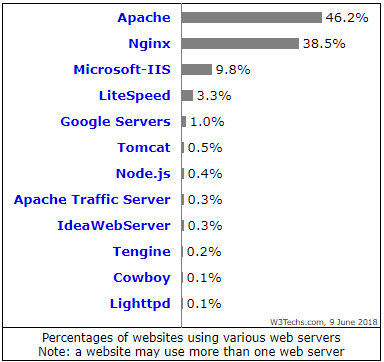
\includegraphics[scale=0.75]{imagenes/web-servers-comparison.png}
	\caption{Comparativa de servidores web.\cite{web-server-usage} \label{fig:figura2}}
\end{figure}

Es inmediato captar la superioridad de Apache\cite{apache} en esta gráfica. Esto es debido a que su lanzamiento 
oficial fue en el año 1996. En esta época no tuvo ningún rival y por tanto se posicionó el primero en el mercado, 
persistiendo aún hoy en día en un gran número de equipos.\\

Sin embargo, en esta lista de servidores todos siguen el esquema tradicional en el que cada petición es atendida 
por una hebra. En la situación actual del desarrollo web, se está optando por una nueva metodología. La programación
asíncrona orientada a eventos. En este tipo de arquitecturas se consigue un mejor rendimiento con un menor coste 
de recursos. El único servidor web que presenta este tipo de arquitectura es Node.js y es por ello por lo que está
ganando popularidad a medida que pasa el tiempo. Su porcentaje de uso aún es bajo debido a que es una tecnología 
bastante nueva y que está ganando popularidad en los últimos años, como podemos comprobar en el siguiente gráfico
de tendencia:

\begin{figure}[H]
	\centering
	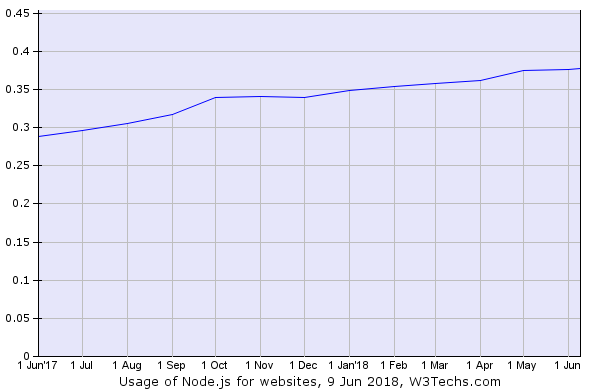
\includegraphics[scale=0.65]{imagenes/nodejs-trend.png}
	\caption{Gráfico de tendencia de Node.js \cite{nodejs-trend} \label{fig:figura2}}
\end{figure}

Además, Node.js dispone de \textit{npm}, que es la herramienta de gestión de paquetes por defecto de Node. Lo impresionante
de este proyecto es la acogida que ha tenido, adquiriendo decenas de miles de usuarios que, además, se involucran
activamente en el desarrollo. Consiguiendo de esta manera la mejora constante del software. Por tanto, se ha conseguido
un gran número de paquetes y hace que el desarrollo con Node sea más liviano dado que podemos utilizar paquetes que 
ha desarrollado la comunidad de una manera muy sencilla.


%Sin embargo, Apache logró su máxima cuota de mercado en el año 2005, siendo usado en el 70\% de los servidores web.
%Desde entonces ha disminuido hasta la cifra actual y según la línea de tendencia continuará descendiendo como podemos
%comprobar en la siguiente gráfica:

%\begin{figure}[H]
%	\centering
%	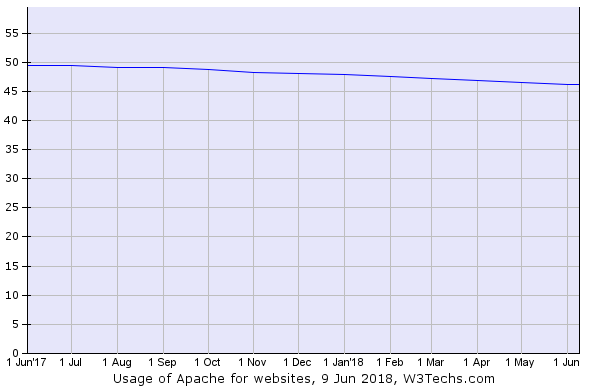
\includegraphics[scale=0.75]{imagenes/apache-trend.png}
%	\caption{tendencia de uso de Apache.\cite{web-server-usage} \label{fig:figura2}}
%\end{figure}


\subsubsection{Elección del lenguaje de programación}
\subsubsection{Elección de la base de datos}

\subsection{Front-end}

\subsubsection{Elección del motor de plantillas} 
\subsubsection{Elección del framework CSS}


Para elegir la tecnología con la que se va a desarrollar el servidor y el \textit{back-end} de la aplicación 
se debe tener en cuenta el uso actual de cada tecnología. En base a 

\section{Solución propuesta}

En base al análisis anterior, la solución al problema planteado se ha conseguido mediante el uso
de las siguientes tecnologías.

% hablar de JSON entre MongoDB y Node.js y por eso MongoDB > SQL

\subsection{Node.js}

Node.js es un entorno de ejecución para JavaScript construido con el motor de JavaScript
V8 de Chrome. En este proyecto se ha utilizado para elaborar el servidor de la aplicación.\\

Node.js tiene una característica que lo diferencia del resto de posibilidades para implementar 
el servidor y es que utiliza un modelo de operaciones E/S sin bloqueo y orientado a eventos 
asícronos. Esto nos ofrece la la posibilidad para que cuando se detecte una conexión se atienda
pero el resto del tiempo estará inactivo. Con este nuevo modelo conseguimos servidores altamente 
escalables de una manera muy sencilla, rápida y eficiente.\\

\begin{figure}[H]
	\centering
	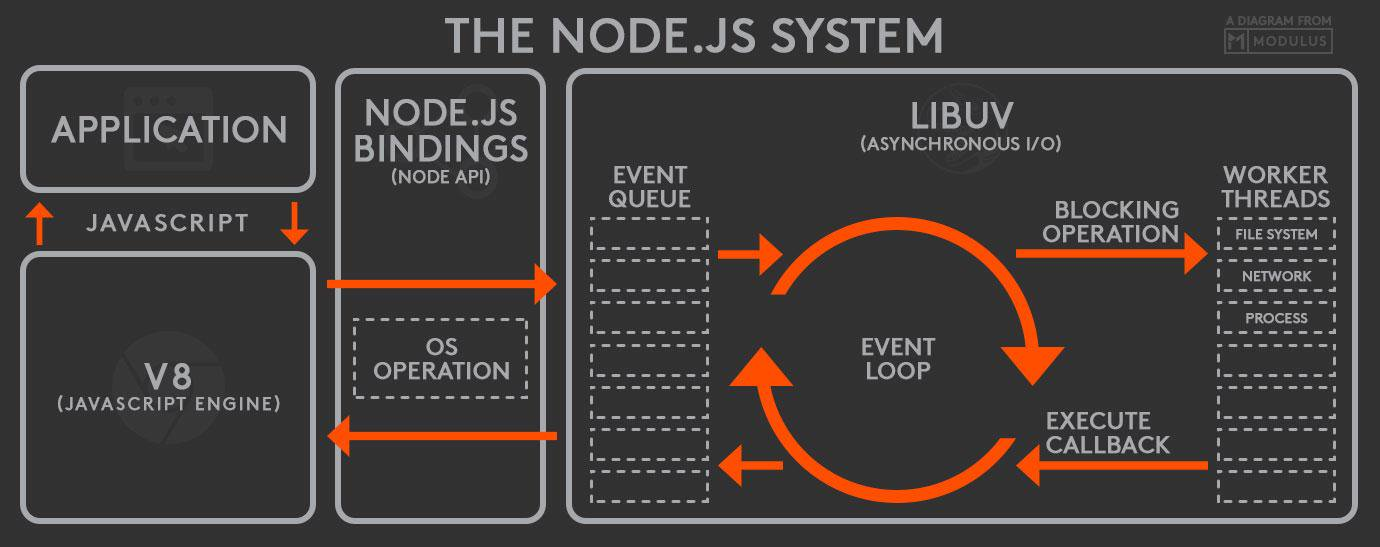
\includegraphics[scale=0.25]{imagenes/nodejs_system.jpg}
	\caption{Sistema de Nodejs \label{fig:figura1}}
\end{figure}

Este diseño contrasta directamente con el modelo con el modelo de concurrencia más común hoy en 
día en el que se usan hilos del Sistema Operativo. Las operaciones en red basadas en este modelo
son relativamente ineficientes además de complejas en su uso. Cabe mencionar que, aunque Node.js 
no utilice hilos del Sistema Operativo implique que no podamos aprovechar los múltiples cores
de nuestro sistema.\\

Otro punto a favor de Node.js es que no tendremos que preocuparnos por la posibilidad de un 
bloqueo en el proceso debido a que no existe dicha posibilidad por la naturaleza de dicha 
tecnología, la cual está basada en un bucle de eventos.

\subsection{MongoDB}

MongoDB es un sistema de base de datos multiplataforma y orientado a documentos de esquema libre.
Esto quiere decir que cada entrada puede tener un esquema de datos diferente al anterior, por
lo que podemos tener entradas que difieran en el número de atributos entre sí.\\

Debido a esta característica los datos no son guardados en registros, como en las bases SQL, 
sino que se guardan en documentos. Estos documentos son del tipo BSON, que es una representación
binaria de los archivos JSON.\\

Esta tecnología ha sido escrita en C++, por lo que está en contacto con el \textit{bare metal}. Esto
último es realmente importante ya que le permite optimizar los recursos y acceder a ellos de una 
manera extremadamente eficiente, con lo que consigue una velocidad muy alta en todas sus operaciones.\\

Cabe mencionar que MongoDB es una plataforma completamente distribuida, lo que nos proporciona 
un nuevo nivel de escalabilidad y disponibilidad. Esto quiere decir que a medida que nuestro desarrollo
crezca tanto en volumen de datos como en rendimiento MongoDB se escala automáticamente sin tiempos
de caída y sin cambios en nuestra aplicación.\\

Por último, cabe mencionar que la licencia de esta tecnología es GNU AGPL 3.0, por lo que se trata de un software de licencia
libre.

% insertar mongodb schema

% gráficas de uso frente al resto de bbdd



\subsection{Vagrant}

Vagrant es una herramienta para construir y administrar entornos de máquinas virtuales de una 
manera sencilla. Debido a que está diseñado para ser sencillo de utilizar y a que se centra en 
la automatización hace que utilicemos el menor tiempo posible en la preparación del entorno virtual
que necesitamos para comenzar a trabajar.\\

Nos proporciona un entorno muy rápido y simple de configurar, reproducible y portable utilizando
tecnología puntera en el sector de la virtualización como puede ser VirtualBox, VMWare, AWS, Docker...\\

Una enorme ventaja que aporta Vagrant al desarrollo es la posibilidad de aislar toda la configuración
del entorno y todas sus dependencias. Además, no tiene que deshacerse de las herramientras de trabajo
a las que está acostumbrado, pues realmente se sigue trabajando en el mismo entorno. 
De esta manera se consigue un desarrollo más eficiente y con mínimas pérdidas de tiempo, garantizando 
de manera directa una eficiencia en la gestión de los recursos humanos empleados.\\

% insertar vagrant advantages


\subsection{Ansible}

Ansible es un software que se ha diseñado explícitamente para automatizar acciones y
conseguir una mayor productividad. De esta manera, se libera al equipo de tareas costosas
y que siempre siguen el mismo proceso.\\

Ansible está categorizado bajo el nombre de \textbf{herramineta de orquestación} debido a 
las funciones que realiza. Se encarga de manejar nodos a través de SSH habiendo recibido
una entrada por parte del usuario. De esta manera, se le entrega una entrada muy sencilla
y comprensible para la lectura del ser humano, que posteriormente es analizada y transformada
en una serie de tareas hacia los nodos, consiguiendo quedar completamente configurados de una
manera muy rápida y sencilla.\\

% insertar ansible workflow

Es la herramienta de automatización de código libre más potente actualmente y esto es reflejado
en las estadísticas de GitHub del proyecto. Además, la comunidad está implicada muy directamente
en el desarrollo de esta herramienta ya que cuenta con más de 2.400 personas que han desarrollado
uno o varios módulos para mejorarla.

\section{Análisis de seguridad}
